\section{Экспериментальное исследование и оценка эффективности программного комплекса}

\subsection{Архитектура пользовательского интерфейса и режимы работы}

Для проведения экспериментальных исследований и наглядной демонстрации работы алгоритма был разработан графический веб-интерфейс. Взаимодействие с системой осуществляется в парадигме клиент-серверного приложения.

В целях снижения когнитивной нагрузки на пользователя и обеспечения гибкости тестирования интерфейс разделен на два функциональных режима, которые представлены на рисунке~\ref{fig:interface_main}:
\begin{enumerate}
    \item «Автоматический режим» скрывает от пользователя сложные математические параметры. Алгоритм маршрутизации самостоятельно вычисляет информационную емкость изображения и назначает оптимальную глубину вейвлет-декомпозиции, а также параметры извлечения цветового паспорта. Данный режим симулирует реальную работу системы на периферийном устройстве конечного пользователя.
    \item «Лабораторный стенд» предоставляет оператору полный контроль над гиперпараметрами кодека. В данном режиме открывается дополнительная панель, позволяющая принудительно задавать уровень каскада вейвлет-преобразования от полного отключения базового алгоритма до экстремального третьего уровня, а также определять разрешение цветового паспорта и плотность контурной карты Кенни.
\end{enumerate}

\begin{figure}[ht]
    \centering
    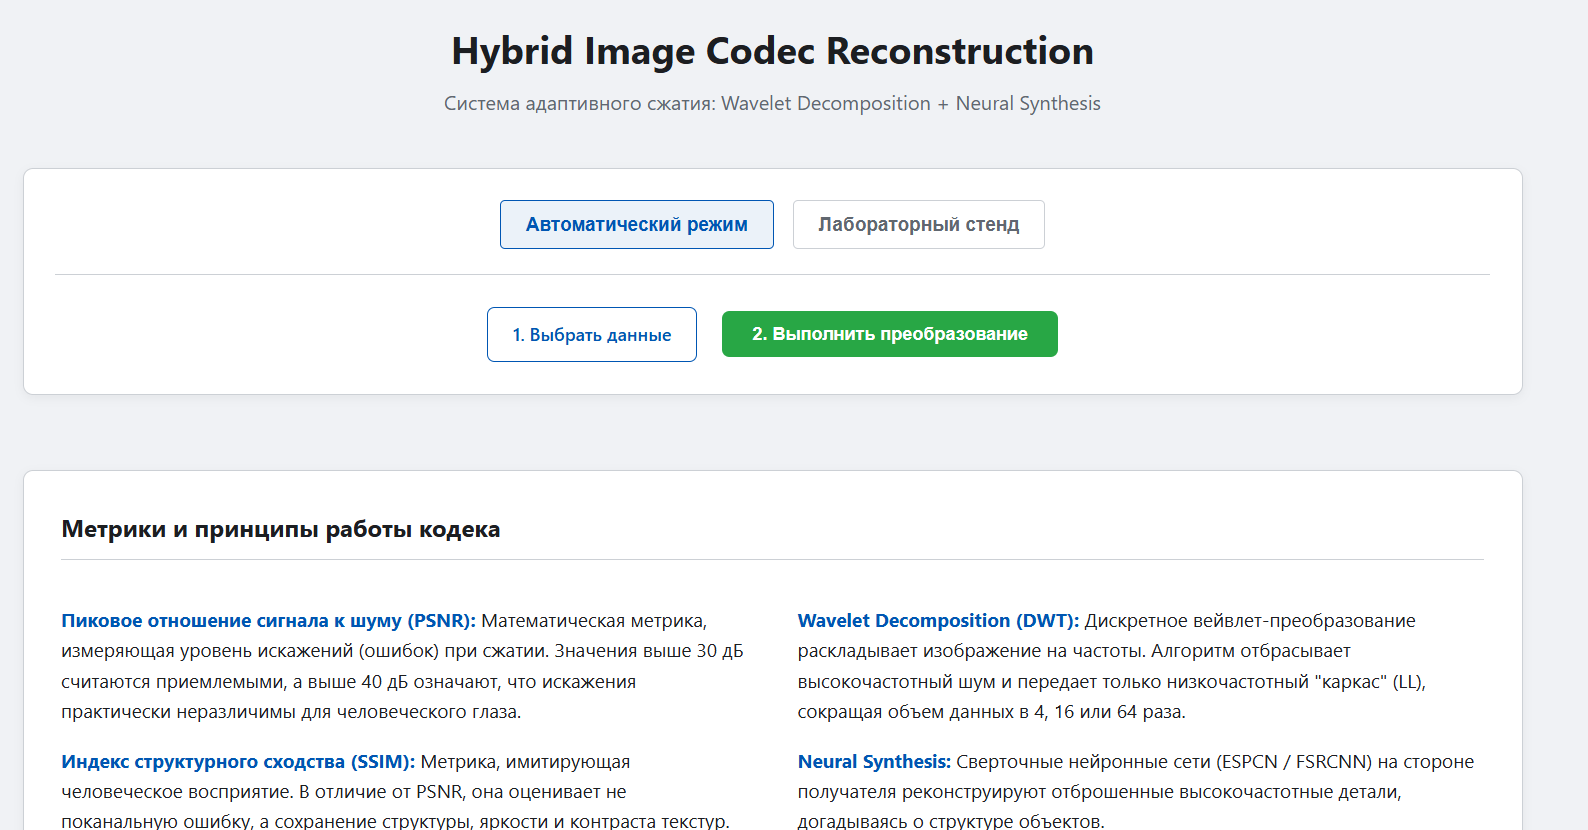
\includegraphics[width=0.85\textwidth]{media/images/interface_main.png}
    \caption{Графический интерфейс лабораторного стенда гибридного кодека}
    \label{fig:interface_main}
\end{figure}

\subsection{Методология тестирования и сравнительный анализ форматов}

Одной из ключевых задач экспериментального исследования является сравнение предложенного гибридного подхода с классическими форматами хранения растровой графики.

Индустриальным стандартом для хранения изображений без потерь является формат PNG. Он гарантирует математическое совпадение декодированного изображения с оригиналом за счет использования алгоритма сжатия Deflate \cite{salomon2004}. Однако платой за отсутствие искажений становится огромный объем генерируемого трафика.

С другой стороны, стандарт JPEG \cite{wallace1992} использует дискретное косинусное преобразование с необратимым квантованием частот. Данный формат способен радикально снизить размер файла, но при высоких степенях компрессии независимая обработка пиксельных блоков приводит к разрушению структуры изображения и появлению хроматических искажений вместе с блочными артефактами в виде ярко выраженных квадратов.

\begin{figure}[ht]
    \centering
    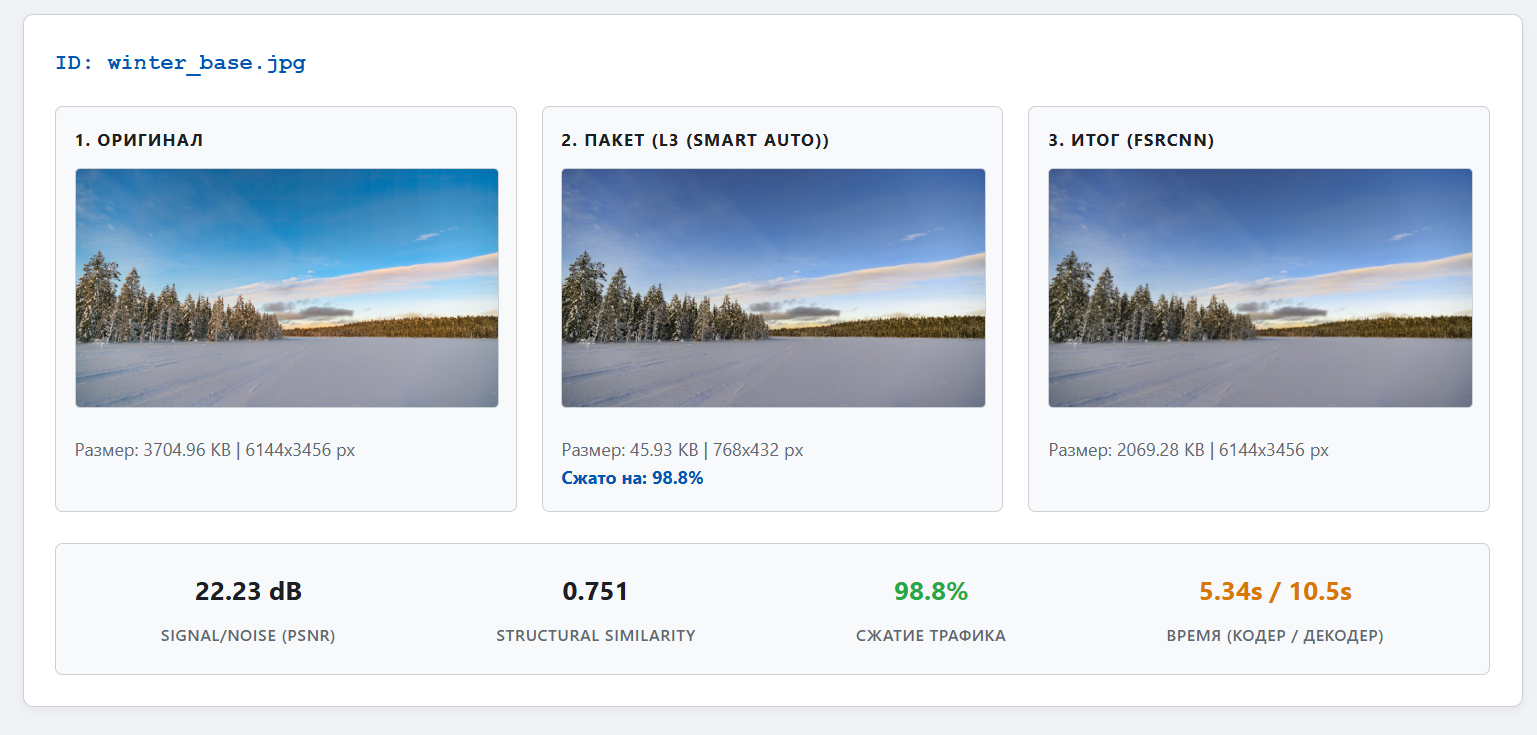
\includegraphics[width=0.9\textwidth]{media/images/interface_results.png}
    \caption{Визуализация этапов гибридной компрессии и нейросетевого восстановления}
    \label{fig:interface_results}
\end{figure}

Разработанный гибридный алгоритм, результаты работы которого представлены на рисунке~\ref{fig:interface_results}, решает конфликт между размером и качеством. Как видно на сетке результатов, исходный тяжеловесный оригинал в формате PNG преобразуется кодером в промежуточный пакет передачи. Этот пакет представляет собой вейвлет-скелет низкочастотной субполосы, инкапсулированный в JPEG-контейнер и дополненный килобайтными метаданными. Визуально пакет выглядит как сильно уменьшенная и размытая копия оригинала, однако его физический размер сокращается на 80--95\,\% по сравнению с исходным файлом.

На третьем этапе формирования восстановленного результата сверточная нейронная сеть на стороне получателя синтезирует высокочастотные детали из переданного каркаса. Итоговое изображение лишено классических блочных артефактов, а переданный цветовой паспорт восстанавливает истинную хроматику, предотвращая феномен нейросетевого галлюцинирования.

\subsection{Оценка метрик объективного качества и вычислительной асимметрии}

Для подтверждения эффективности системы был проведен анализ объективных математических метрик. Результаты тестирования выводятся в специализированной панели интерфейса, показанной на рисунке~\ref{fig:interface_metrics}.

\begin{figure}[ht]
    \centering
    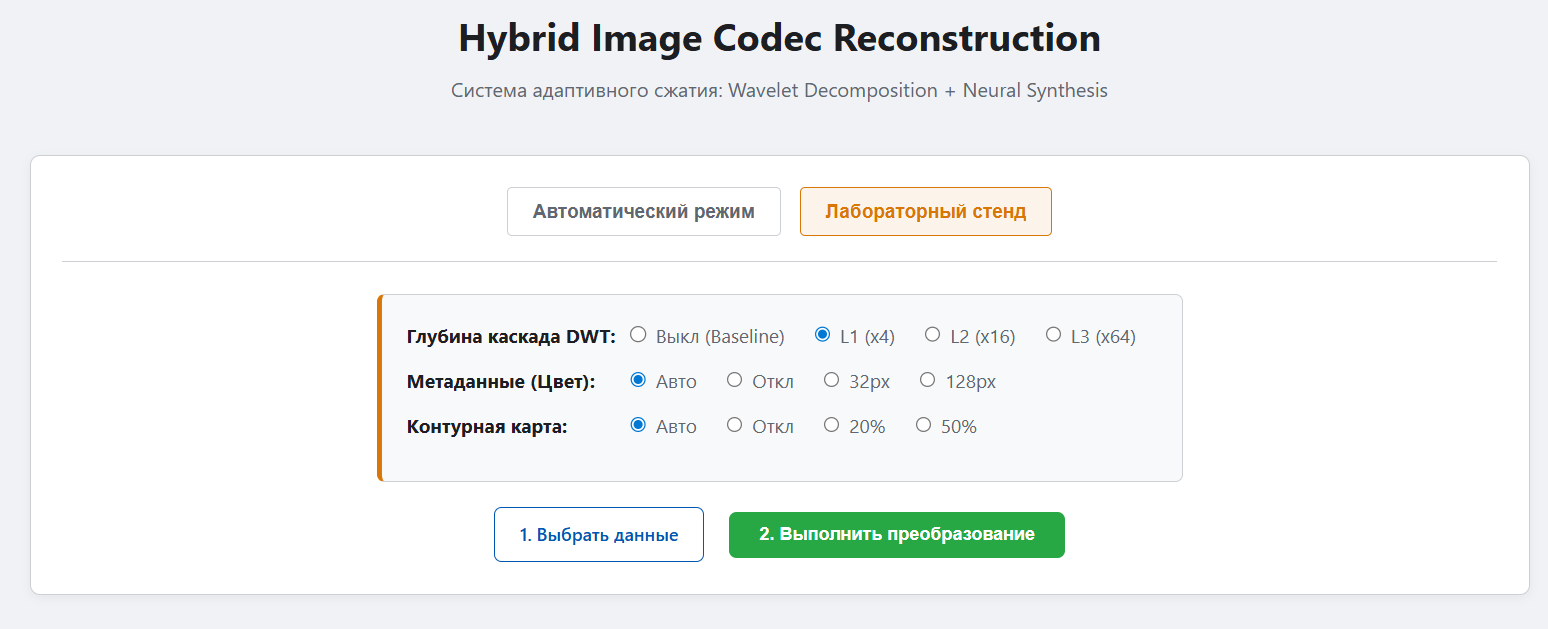
\includegraphics[width=0.9\textwidth]{media/images/interface_metrics.png}
    \caption{Панель объективного контроля качества и временных характеристик алгоритма}
    \label{fig:interface_metrics}
\end{figure}

Эксперименты показали, что при экстремальных коэффициентах сжатия трафика метрика PSNR \cite{gonzalez2012} стабильно превышает порог в 30~дБ, что свидетельствует о низком уровне среднеквадратичной ошибки MSE. Индекс структурного сходства SSIM \cite{wang2004ssim} достигает значений 0,85--0,95, что означает высокую психовизуальную идентичность восстановленного кадра оригиналу.

Процесс кодирования DWT и извлечения метаданных на стороне отправителя занимает миллисекунды. Поэтому алгоритм идеально подходит для слабых мобильных процессоров, экономя заряд батареи. Процесс реконструкции на стороне декодера использует многопоточный тензорный инференс и занимает в разы больше времени, однако эта нагрузка штатно делегируется мощному удаленному серверу, что доказывает успешную реализацию парадигмы Edge-to-Cloud.

Для проведения комплексного сравнительного анализа эффективности разработанного решения было выполнено построение кривых зависимости уровня искажений от битрейта \cite{bovik2009}. В качестве тестового набора данных использовался пакет из 4~изображений. Сравнение проводилось с индустриальными стандартами: JPEG, WebP и JPEG 2000. Результаты эксперимента, визуализированные с помощью библиотеки Matplotlib \cite{hunter2007matplotlib}, представлены на рисунке~\ref{fig:rd_curve}.

\begin{figure}[ht]
    \centering
    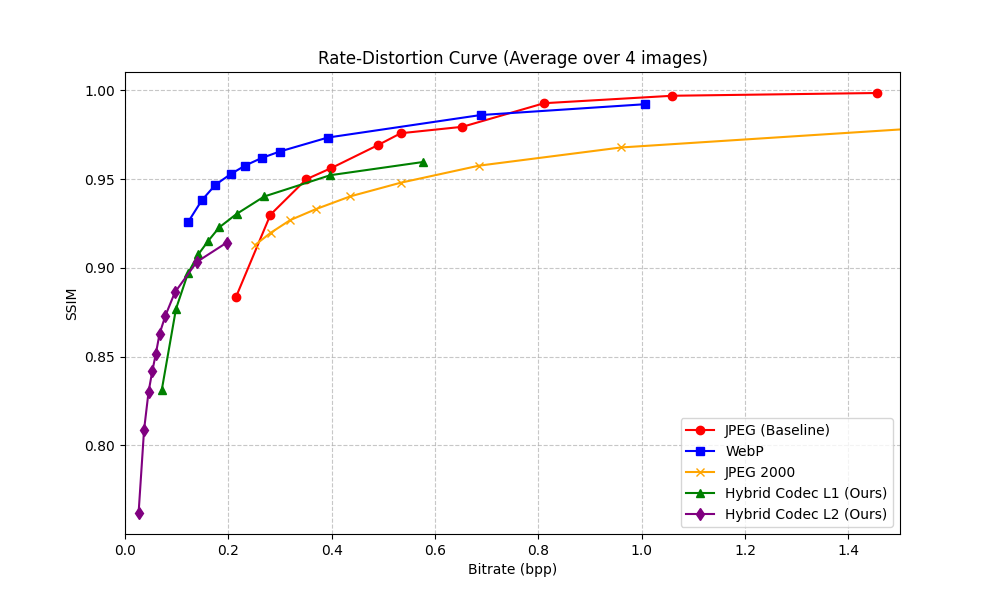
\includegraphics[width=0.95\textwidth]{media/images/rate_distortion.png}
    \caption{Сравнительный анализ зависимости SSIM от битрейта}
    \label{fig:rd_curve}
\end{figure}

Анализ экспериментальных данных позволяет сделать следующие выводы:
\begin{enumerate}
    \item В зоне экстремально низкого битрейта (менее 0,1~бит/пиксель) форматы JPEG и WebP физически не способны обеспечить сжатие. Стандарт JPEG 2000 достигает минимальной отметки $\approx 0,2$~бит/пиксель, показывая структурное сходство на уровне SSIM $\approx 0,85$. В то же время гибридный кодек (L2) уверенно функционирует при вдвое меньшем битрейте ($\approx 0,1$~бит/пиксель), сохраняя при этом высокий показатель SSIM $\approx 0,85\text{--}0,90$.
    \item Гибридный алгоритм (L1) достигает высокого психовизуального сходства (SSIM $\approx 0,92$) при битрейте $\approx 0,18$~бит/пиксель. По графику видно, что для достижения аналогичного качества (при SSIM, равном 0,92) стандарту JPEG 2000 требуется битрейт около $0,3$~бит/пиксель, а классическому JPEG --- порядка $0,3$~бит/пиксель. Это подтверждает превосходство предложенного метода в эффективности использования пропускной способности канала связи.
    \item Вертикальная ориентация кривых гибридного кодека (в отличие от пологих графиков классических форматов) наглядно доказывает асимметричную природу алгоритма: основной прирост визуального качества обеспечивается не за счет увеличения веса передаваемого пакета данных (движение по оси X), а за счет вычислительного синтеза нейронной сети на стороне приемника (вытягивание по оси Y).
\end{enumerate}